\documentclass[a4paper, 12pt]{article}

%----------------------Packages généraux------------------------------

\usepackage[french]{babel}
\usepackage[T1]{fontenc}
\usepackage{ae}
\usepackage[utf8]{inputenc}
\usepackage{vmargin}
\usepackage{hyperref}

%\setmarginsrb{1.75cm}{1cm}{1.75cm}{1cm}{1cm}{0.5cm}{1cm}{0.5cm}
%1 est la marge gauche
%2 est la marge en haut
%3 est la marge droite
%4 est la marge en bas
%5 fixe la hauteur de l'entête
%6 fixe la distance entre l'entête et le texte
%7 fixe la hauteur du pied de page
%8 fixe la distance entre le texte et le pied de page

%----------------------------Mathématiques----------------------------

\usepackage{amsmath}
\usepackage{amssymb}
\usepackage{amsthm}
\usepackage{amsfonts}
\usepackage{eucal}



%------------------------------Graphics------------------------------

\usepackage{comment}
\usepackage{graphicx}
\usepackage{fancyhdr}
\usepackage{fancybox}
\usepackage{color}
\usepackage{epstopdf}
\usepackage{float}
\usepackage{diagbox}
\usepackage[justification=centering]{caption}
\usepackage{float}
\usepackage{tikz}
\usepackage{subcaption}

%------------------------------Syntaxe------------------------------

\usepackage{listings}
\lstloadlanguages{C}

\setlength{\parindent}{0.5cm}
\setlength{\parskip}{1ex plus 0.5ex minus 0.2ex}
\newcommand{\HRule}{\rule{\linewidth}{0.5mm}}


\definecolor{mygreen}{rgb}{0,0.6,0}
\definecolor{mygray}{rgb}{0.5,0.5,0.5}
\definecolor{mymauve}{rgb}{0.58,0,0.82}
\usepackage{enumitem}
\setlist[itemize]{topsep = 3pt}

\lstdefinestyle{customc}{
  belowcaptionskip=1\baselineskip,
  breaklines=true,
  frame=L,
  xleftmargin=\parindent,
  language=C,
  showstringspaces=false,
  basicstyle=\footnotesize\ttfamily,
  commentstyle=\color{mygreen},
  frame=single,	
  keywordstyle=\bfseries\color{mymauve},
  commentstyle=\itshape\color{mygreen},
  identifierstyle=\color{blue},
  stringstyle=\color{mygray},
}
\lstset{escapechar=@,style=customc}

%Nouvelles commandes
%double souligné
\newcommand{\Bo}{\underline{\underline{B_0}}}
\newcommand{\Ko}{\underline{\underline{K_0}}}
\newcommand{\xo}{\underline{x_0}}
\newcommand{\x}{\underline{x}}

\newcommand{\Bel}{\underline{\underline{B_{el}}}}
\newcommand{\Kel}{\underline{\underline{K_{el}}}}
\newcommand{\B}{\underline{\underline{B}}}
\newcommand{\dK}{\Delta\underline{\underline{K}}}
\newcommand{\II}{\underline{\underline{I}}} %Matrice unitaire I

\newcommand{\I}{\int\limits_0^L}
\newcommand{\SigA}{\sigma_{\alpha}}
\newcommand{\AutoCor}{\sigma_{\alpha}^2 e^{\frac{-|\Delta(s)|}{l}}}
\newcommand{\IntEspCor}{2\sigma_{\alpha}^2\frac{l^2}{L^2}\left(e^{\frac{-L}{l}}+\frac{L}{l}-1\right)}
\newcommand{\EspAlpha}{-\sigma_{\alpha}^2+2\sigma_{\alpha}^2\frac{l^2}{L^2}\left(e^{\frac{-L}{l}}+\frac{L}{l}-1\right)}
\newcommand{\OU}{\text{ }|\text{ }}

\newcommand{\png}[3]{\begin{figure}[H]
    \centering
    \includegraphics[scale = 0.33]{#1.png}
    \caption{#2}
    \label{#3}
\end{figure}}

\newcommand{\myref}[2]{\href{#1}{\textcolor{blue}{\underline{#2}}}}

\newcommand{\tab}[1]{\hspace{.022\textwidth}\rlap{#1}}

\begin{document}

\begin{titlepage}

  	\begin{center} 

    	% top part of the page. The '~' is needed because \\
    	% only works if a paragraph has started.
	
    
\includegraphics[scale=0.35]{logo_fsa.png}  %A changer : image hec
    
\includegraphics[scale=0.6]{logo_Ulg.png}\\[1.15cm]
   		\textsc{\Large First Version}\\[1.2cm]

    	% Title
    	\HRule 
    	\\[0.4cm]
    	{\bfseries \LARGE     Master Thesis
    	\\[0.4cm] 

    	\HRule} \\[2cm]
    	

  
 
    % Author and supervisor
    \begin{minipage}{0.4\textwidth}
      \begin{flushleft} \large
         Stassen Théo (s150804)
      \end{flushleft}
    \end{minipage}
    \begin{minipage}{0.4\textwidth}
      \begin{flushright} \large
        \emph{Promoter :} D. Ernst \\      
      \end{flushright}
    \end{minipage}

    \vfill

    % Bottom of the page
    \large 2019-2020

  \end{center}
\end{titlepage}

\newpage


\section{Context} \label{intro}

Blacklight Analytics is a enterprise that develop solutions regarding the management of electrical distribution networks. 
Distribution systems
need to integrate more and more renewable generation in their network. Since networks cannot be quickly upgraded and at low cost, new generators are connected to the network under non-firm access contract. The assets used in networks have been designed to transmit power in one direction, from the global network to the local network. This configuration implies situations where the high production creates congestion problems in the assets, while energy generated must be injected into the global network . There is
a need for a practical method able to compute the production limits of the generators such that the system can be considered safe, i.e has a low probability that the electrical power flowing through one asset is higher than the maximum tolerated power is this asset.


Blacklight Analytics develops a solution to 
this problem. The method cast the problem into a stochastic decision process. This process is divided in three phases : (i) generation of a network model, (ii) forecasting of the power produced or consumed and (iii) computation of the generator limits. The phase 2 takes as input historical measurements of the networks and output future production probability distribution for each sources. This output will be used to define generator limits.
In the current implementation, the forecasting method uses Gaussian process regression to forecast individually each source and combine information using covariance estimation. 
This master thesis subject addresses the question of what is the best forecasting method to implement in this described context, and what are the elements of comparison that allows us to make these affirmation. The growing scientific field of Deep Learning has a great potential to be exploited to achieve this goal. 



Therefore, the concrete goal of this Master Thesis is the comparison of different probabilistic forecasting models and techniques, mostly from the deep learning scientific field,
in the context of the prediction of renewable energy production.


Regarding the technical aspect of the Master Thesis, the main working tool 
is GluonTS, a toolkit for probabilistic time series modeling, focusing on deep learning-based models and relying on the deep-learning framework MXNet, developed by Amazon.


\subsection{General Problem Statement}

Before entering into solution description, we need to define mathematically in general the problem of time series deep-learning forecasting, whereabouts GluonTS has been conceived. 
Depending of the type of model used, there are some significant differences in expressions. 
Two main cases are presented, the feed-forward models case (which belongs to the generative models category) and the RNN models case (which belongs to the discriminative models category).
The neural network need at least one time series. A part is visible during training and testing ( $0\leq t<pf$) and a part is visible only during testing ($pf\leq t < ef$).
 In contrast to classical model approach like ETS and ARIMA, which consider functions per time series individually, neural models further express one function, as a neural network, whose weights are trained among all time series given as input and learned from the whole training data. Each time series can be tested using this trained neural network.

\subsection{Feed-forward case}

\begin{center}
\begin{tikzpicture}
\draw (0,0) -- (0,3);
\draw (10,0) -- (10,3);
\draw (0,0) -- (10,0);
\draw (0,3) -- (10,3);
\draw [very thin, blue] (3,0) -- (3,3);
\draw [very thin, cyan] (6,0) -- (6,3);
\draw [very thin, blue] (7,0) -- (7,3);
\draw [red] (9,0) -- (9,3);
\draw (0,1.5) node [left] {$x$};
\draw (0,3) node [above] {$0$};
\draw (3,3) node [above] {$c$};
\draw (6,3) node [above] {$p$};
\draw (7,3) node [above] {$e$};
\draw (9,3) node [above] {$pf$};
\draw (10,3) node [above] {$ef$};
\draw [<->, blue] (2.5,1.5) -- (3,1.5);
\draw [<->, blue] (7,1.5) -- (7.5,1.5);
\draw [help lines, dashed,ystep=10] (0,0) grid(10,3);
\end{tikzpicture}
\end{center}

Training function statement : 

\begin{equation}
    [\phi_{x_p},..,\phi_{x_{e-1}}] = f({x_c},..,{x_{p-1}}), \forall c \in [0, pf-(e-c)]
\end{equation}

f is the training function, implemented as a neural network.
With $x_t$ the variable representing energy production at time step t, $\phi_{x_t}$  the density of probability of $x_t$. With $0<c<p<e<pf<ef$. 
$predict\_length = p-c$ and $context\_length = e-p$ are hyper parameters of the problem. 

Training loss statement :


\begin{equation}
    loss = \sum^{e-1}_{t=p}l(x_t,\phi_{x_t})
\end{equation}

l is the chosen loss taking a x value and a density of probability as input.
The details of loss implementation are discussed in section \ref{loss}, the loss choose coming from
the discussion about project goal in section \ref{goal}.

Testing function statement :

\begin{equation}
    [\phi_{x_{pf}},..,\phi_{x_{ef-1}}] = f(\phi_{x_{pf-(p-c)}},..,\phi_{x_{pf-1}})
\end{equation}

\begin{equation}
    metrics([\phi_{x_{pf}},..,\phi_{x_{ef-1}}],{x_{pf}},..,{x_{ef-1}})
\end{equation}

The details of metrics function are discussed in section \ref{metrics}

\subsection{RNN case}

\begin{center}
\begin{tikzpicture}
\draw (0,0) -- (0,3);
\draw (10,0) -- (10,3);
\draw (0,0) -- (10,0);
\draw (0,3) -- (10,3);
\draw [very thin, blue] (3,0) -- (3,3);
\draw [very thin, blue] (7,0) -- (7,3);
\draw [red] (9,0) -- (9,3);
\draw (0,1.5) node [left] {$x$};
\draw (0,3) node [above] {$0$};
\draw (3,3) node [above] {$c$};
\draw (7,3) node [above] {$e$};
\draw (9,3) node [above] {$pf$};
\draw (10,3) node [above] {$ef$};
\draw [<->, blue] (2.5,1.5) -- (3,1.5);
\draw [<->, blue] (7,1.5) -- (7.5,1.5);
\draw [help lines, dashed,ystep=10] (0,0) grid(10,3);
\end{tikzpicture}
\end{center}

Training function statement : 

\begin{equation}
    [\phi_{x_c},..,\phi_{x_{e-1}}] = f({x_c},..,{x_{e-1}}, {h_c},..,{h_{e-2}}), \forall c \in [0, pf-(e-c)]
\end{equation}

With $x_t$ the variable representing energy production at time step t, $\phi_{x_t}$  the density of probability of $x_t$, $h_t$ the state variable at time step t. With $0<c<e<pf<ef$, $predict\_length + context\_length  = e-c$.

Training loss statement :


\begin{equation}
    loss = \sum^{e-1}_{t=c}l(x_t,\phi_{x_t})
\end{equation}

l is the chosen loss with a value and a density of probability as input.

Testing function statement :
\begin{equation}
    \phi_{x_{pf}} = f(\phi_{x_{pf-1}},h_{pf-1})
\end{equation}
\begin{equation}
    \phi_{x_{pf+1}} = f(h_{pf},\phi_{x_{pf}} )
\end{equation}
\begin{equation}
    [\phi_{x_{pf}},..,\phi_{x_{ef-1}}] = f(\phi_{x_{pf-1}},h_{pf-1},..,h_{ef-2})
\end{equation}
\begin{equation}
    metrics([\phi_{x_{pf}},..,\phi_{x_{ef-1}}],{x_{pf}},..,{x_{ef-1}})
\end{equation}



\section{Solution}

GluonTS forecasting process is composed of different parts.
The toolkit defines a dataset structure , containing in particular the time series describing a stochastic process. This dataset is given to a GluonTS model (pre-implemented or implemented using model template) , which consider this dataset information as input for his network and gives as output a forecast sampled distribution density of each of the future time steps (the type of output distribution is defined by the user and discussed in this paper). Concretely the output information is a set of sample of the predicted distribution,
not the distribution parameters or density itself.
This network, if using deep learning, must be trained before evaluate, using a certain loss.
The resulting distribution can be studied and evaluate using the appropriate tools (metrics).

\subsection{Datasets}

GluonTS interface imposes a certain structure of datasets, object used for training and testing models. There are composed of some mandatory and some optional components.
$`dataset.train`$ is an iterable collection of data entries used for training. Each entry corresponds to one time series.  $'dataset.test$ is an iterable collection of data entries used for inference.
In the classical way of declaring a dataset object, test dataset is constructed on the same time series than training dataset, as  the test dataset is an extended version of the train dataset that contains a window in the end of each time series that was not seen during training. This window has length equal to the prediction length. $`dataset.metadata`$ contains metadata of the dataset such as the frequency of the time series, the context (training) length,  the prediction length and associated features. These features are data given in addition to the time series information, that will also been seen as input by the network. They can be static, dynamic, real, categorical , etc.

We should emphasize here that a single moded is trained over all the time series contained in the training dataset . This results in a global model, suitable for prediction for all the time series in the testing dataset as it is defined in the classical way and possibly for other unseen related time series.

GluonTS is optimized to handle multiple time series in parallel. A dataset composed of only one time serie of very long length will make the model training really slow.

In the current implementation, the input dataset (training and testing, in the classical way of using datasets) is construct on one time serie describing the production of one wind turbine generator during 6 month, with a 1 minute frequency. This time series is manually splitted in certain number of samples. The time series is currently splitted in days, resulting in a training/testing set composed of 183 time series of size 1440, but other split size could be explored as a hyper-parameter of the problem. 
In practical application of the model, the training data at our disposal will be different time series corresponding to different renewable energy generator sources. All this series will be considered as one only dataset, with associated features identifying the different sources, for example the type or the nominative power of each source as static categorical feature.  The testing data will be a different source. The training and testing datasets will not be constructed on the same time series.

The size of the prediction window we are interested in is 10 minutes, i.e 10 time steps.
The model output sampled distribution for each of these time steps. 



\subsection{Goal definition and quantiles} \label{goal}

The third step of the stochastic decision process described in section \ref{intro} is, more than everything, interested in a forecasting that gives a precise estimation of the value of production for which there is a very low probability (value that could be discussed) that the production in the given time window outnumber this value. That value will be called the "security limit" and will be used to determine, knowing what is the maximum acceptable production value, if the generator limits must be modified.
In other terms, considering that the model output is a distribution with it density of probability, the goal fixed is not to minimize the difference (in any ways to define it) between the predicted and observed time series but to minimize the difference between the predicted "security quantile", i.e the $quantile(1-e)$ of the predicted distribution, knowing that $e$ is the probability of error considered as acceptable, and the real security quantile (the quantile of the real probability distribution of the source).
A too low predicted security quantile signify that the risk of production oversupply is underestimated,
leading to situation where the system will estimate that the network is safe wrongly. 
Inversely a too high predicted security quantile signify that the risk is overestimated, leading to situations where the production limit will be decreased unnecessarily. This situation is nevertheless less problematic than the first one.
This minimization must be for all time steps of the prediction range. 
This objective is not disconnected from the classical objective consisting in minimizing the difference. 
If the predicted model understand well the unknown process, and gives a distribution close to the reality, the quantiles will be close to the reality.


GluonTS allow selecting the values of quantiles that will be computed, to evaluate the metrics and to possibly use these information in loss function.
In current implementation, the value of $e$ is $1\%$ but the security quantile is $quantile(0.995)$ because of a little modification comparing to the goal specified before. The goal currently considered is not only the difference minimization of the "upper" quantile but also the reverse "lower" quantile, concretely $quantile(0.995)$ and $ quantile(0.005)$, in order to obtain a 99\% window as correct as possible. It impacts the formulation of the custom loss and custom metric in respective sections. This must probably be modified to focus only on the $quantile(0.99)$.
  
  \subsection{Custom Loss} \label{loss}

Considering that, as we have seen in section \ref{goal}, the model training follow an non-traditional goal, the loss function must be discussed.

GluonTS implements in it predefined models only one type of loss, the inverse of the log-density of the the output distribution. 
If $ \mu $ and $ \sigma $ are the parameters of the distribution output (in the case of a gaussian) of the model and x the observed value of production, the loss value of x is : 

\begin{equation}
    base\_loss(x, \varphi ) = - ln \varphi_{\mu,\sigma^2}(x)  
\end{equation}

This loss express efficiently that the predicted distribution must corresponds to the real distribution.
It penalize a too large or too thigh quantile window compared to the real window.
Nevertheless, it doesn't penalize much the main priority which is the risk underestimation case (too tight window). Concrete results will confirm that if used loss is base loss, models tends to underestimate the risk. 

\begin{figure}[!h]
    \centering
    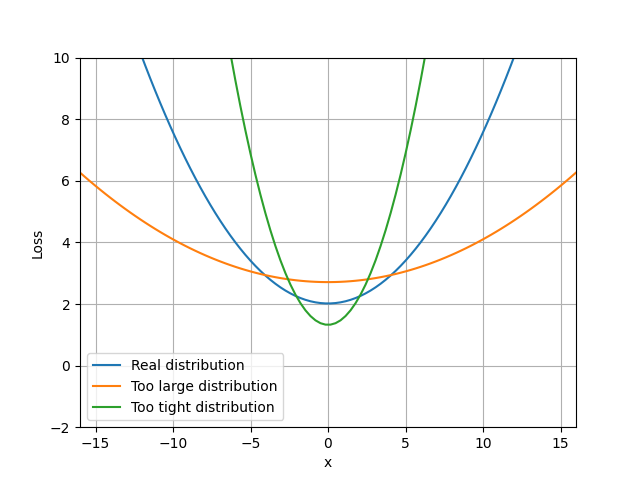
\includegraphics[width=400px]{distribution_comp.png}
    \caption{Comparison of the real distribution loss, a too large predicted distribution window and a too tight distribution window}
    \label{fig:distrib_comp}
\end{figure}

To tackle this problem, another loss function is needed to penalize values of x bigger than $quantile(0.99)$ (and lower than 
$quantile(0.01)$ )
The proposed loss is the following (with $e = 0.01$):

\begin{equation}
    alt\_loss(x,\varphi ) = e^{x - quantile_\varphi (0.995)} + e^{quantile_\varphi (0.005)-x}
\end{equation}


The loss increase exponentially if x is outside the security window, and is remains low if x is in the window.
The defined objective cannot be expressed literally as the quantile of the real distribution is unknown.
This loss express indirectly the objective that has been fixed, by penalising heavily the model when observed values are outside the security window, indicating that the window is too small. 
The opposite situation (window too large) is handle by the base loss, as this situation results in a higher loss, in mean.
See \ref{fig:distrib_comp}.


The only way to use other loss than the base loss in GluonTS is to define custom models, based on the original but with intern modifications to change loss function.

At this time, three custom models (one original, \textit{"Simple"}, and the copy of the pre-implemented \textit{"SimpleFeedForward"} and 
\textit{"CanonicalRNN"}) are implemented. The loss implemented in these custom model is the following :

\begin{equation}
    custom\_loss(x,\phi ) = base\_loss(x,\phi ) + \alpha * alt\_loss(x,\phi )
\end{equation}


\begin{figure}[!h]
    \centering
    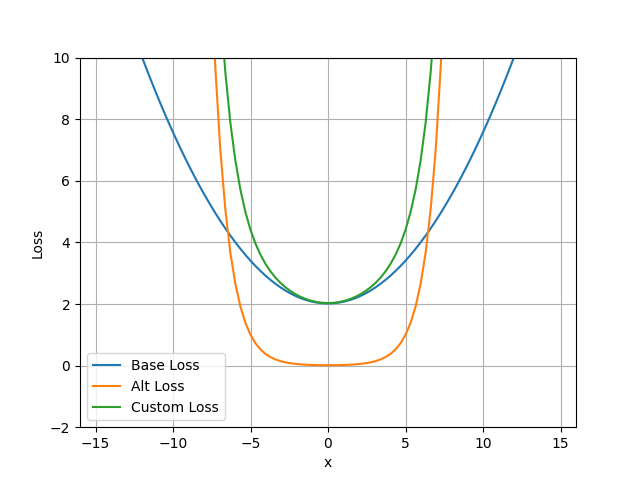
\includegraphics[width=400px]{base_loss_vs_custom_loss.png}
    \caption{Comparison of Base Loss, Alt Loss and Custom Loss, with x the difference between the observed value and
    the median of the predicted distribution}
    \label{fig:customloss}
\end{figure}

With $\alpha$ a parameter with a great impact on the results. It value will be subject of comparison.

  
  
\subsection{Metrics} \label{metrics}

Concerning the evaluation of the results, GluonTS provides a module using the trained model and testing data to provide quantitative results, as metrics (global, for all time series, or unit, for each series separately). Metrics proposed by GluonTS includes MSE, MSIS, RMSE, and other classical measures.
Knowing the goal pursued, the main needed metric must indicates if the predicted quantiles are over/under-estimated. 
The proposed 
metric, \textit{"Coverage"} uses an implemented metric, $coverage(x)$.
This metric gives the observed probability having a value below $quantile(x)$.
For $e=0.01$ :  
\begin{equation}
    Coverage = (0.01 - coverage(0.005)) + (coverage(0.995) - 0.995) 
\end{equation}

The Coverage of the predicted distribution must tends to 0 to achieve the goal. For the upper quantile,
if coverage(0.995) > 0.995, the quantile is too high (the window is too large) and
if coverage(x) < x the quantile is too tight.


In addition, another useful indicator is how much the output probability distribution is spread out. 
A proposed metric is  the mean of the difference between 
the quantile(0.995) and quantile(0.005) values. For a time series :

\begin{equation}
    Bandwidth = \frac{1}{T}  \sum_{t=0}^{T-1} quantile_{t}(0.995) - quantile_{t}(0.005) 
\end{equation}


Where T is the number of time step and $quantile_{i}$ the value of the quantile at time step t


\subsection{Distribution}\label{distribution}

GluonTs proposes different type of output distribution. In most of the models the output is technically
 a vector of values which is
transformed to a vector of distribution parameters  and put in a distribution object.
In current implementation, three of them are functional. $Gaussian$, $Laplace$ and $PiecewiseLinear$.
$Student$ has been rejected because the quantiles of the distribution are not obtainable.
$Uniform$ has been rejected because of loss problems in execution.
Other options are available, as multiple kernel gaussian.
The GluonTS models are mandatory to output an object containing sample of the distribution, not the distribution itself (parameters values). Considering that the parameter information could also be useful, as asked by the client, a modification done in custom models allows saving these information.

\begin{figure}
    \centering
    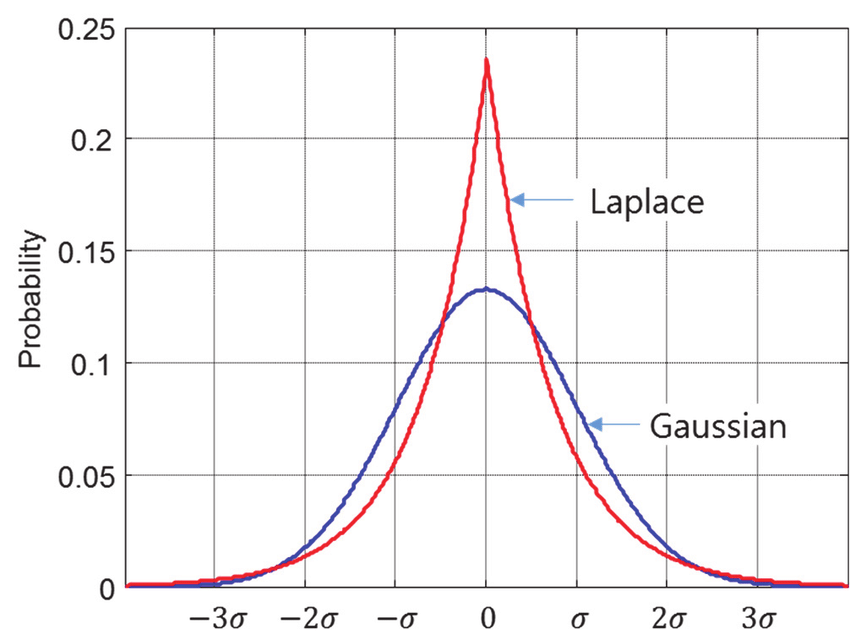
\includegraphics[width=200px]{Gaussian-distribution-and-Laplace-distribution.ppm.png}
    \caption{Comparison between Gaussian distribution and Laplace distribution}
    \label{fig:gausslaplace}
\end{figure}

\begin{figure}
    \centering
    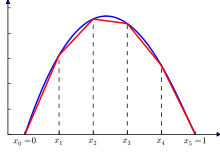
\includegraphics{220px-Finite_element_method_1D_illustration1.svg.png}
    \caption{Comparison between Gaussian distribution and PiecewiseLinear distribution}
    \label{fig:gausslaplace}
\end{figure}

\subsection{Different Models} \label{diff_models}


All the pre-implemented deep learning models that have been tested  are presented here.
They have been trained with different output distribution, $\alpha$ value of custom loss (if custom loss implemented) and with different values of tunable parameters mentioned in each section.
Some global hyper parameters have not been tested : The size of the input time series, the size of training batch, the learning rate, the number of batches per epochs, the context length.



\subsubsection{Simple} \label{descr_simple}
A model which uses a simple 2 fully connected layers neural network.
The tunable parameter is the number of cells in layers.

\subsubsection{FeedForward} \label{descr_feedfordward}
A simple MLP (multi-layer perceptron) model.
The tunable parameter is the number of hidden nodes in each layer.

\subsubsection{Recurrent Neural Network} \label{descr_canonicalRNN}
A model which uses a recurrent neural network.
The tunable parameters are the number of layers and number of cells of the network

\subsubsection{DeepAr} \label{descr_deepar}
Implementation of DeepAr estimator, a RNN based model, close to the one described in paper 
\textit{"DeepAR: Probabilistic Forecasting with Autoregressive Recurrent Networks"} (\url{https://arxiv.org/abs/1704.04110})
The tunable parameters are the same than for CanonicalRNN.

\subsubsection{Deep Factors} \label{descr_deepfactor}
Implementation of the 2019 ICML paper “Deep Factors for Forecasting” (\url{https://arxiv.org/abs/1905.12417}).
Uses a global RNN model to learn patterns across multiple related time series and an arbitrary local model to model the time series on a per time series basis. 
In the current implementation, the local model is a RNN (DF-RNN).
The tunable parameters are the number of units per hidden layers and the number of layers in the global model, the number of units and layers in the local model
, the number of global factors.

\subsubsection{Gaussian Process} \label{descr_gp}
Model using Gaussian Processes (GP).
Each time series has a GP.
There are no parameters easily tunable.

\subsubsection{NPTS} \label{descr_npts}
Implementation of the Non-Parametric Time Series Forecaster, 
which falls into the class of simple forecasters that use one of the past observed targets as the forecast for 
the current time step. It randomly samples a past time index as the prediction for the time step T (auto regressive model, which predict step by step).
There are no parameters to tune, but it exists some variants.

\subsubsection{MQCNN} \label{descr_mqcnn}
Discriminative Sequence to Sequence model made using the \textit{SeqtoSeq} framework of GluonTS to reproduce the model of the 
paper "A Multi-Horizon Quantile Recurrent Forecaster" (\url{https://arxiv.org/abs/1711.11053}).
Sequence to sequence models are composed of two parts. The encoder network, that reads in a certain context of the training range of the time series 
and encodes information about  the  sequence  in  a  latent  state.
And the decoder network, which generates the forecast by combining the latent information with the features in the prediction range.
In MQCNN, the encoder is a Convolutionnal Neural Network and the decoder an MLP. Unlike other models, The output is not technically a distribution but the quantiles itself, that are predicted values obtains by optimizing the corresponding quantile loss.
The tunable parameter is the  dimension of the MLP decoder.
Considering the fundamental difference in the intern functioning, it not seems to be possible to modify the loss as it was modified for the other models.

\subsubsection{MQRNN} \label{descr_mqrnn}
Same as MQCNN but with a Recurrent Neural Network encoder instead.

\subsection{Model comparison}

All the implemented models has been tested individually and collectively. 
Some models gives significantly better results for the moment (more testing is needed).
Two hyper-parameters values as been tested for all models, the value of $\alpha$, and the type of distribution.
A global remark is that $\alpha$ modify a lot the results in term of metrics. The value of \textit{bandwidth } and \textit{Coverage} is proportional to $\alpha$ value, which is in agreement with theory.

\section{Implementation and Results}

\subsection{Testing protocol definition}

Each comparison is presented using as element of comparison the metrics defined in section \ref{metrics}
The plot results are all presented with the same values of quantiles of the the predicted distribution, along the predicted window.

\subsection{Different Configurations of dataset}

\subsection{Hyperparameters comparison}

\subsubsection{Learning rate} \label{comp_lr}

\begin{figure}[!h]
    \centering
    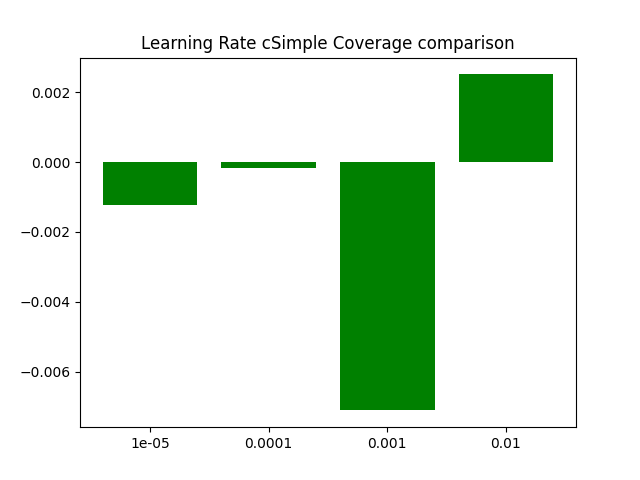
\includegraphics[width=200px]{plots/hist/a/lr/cSimple/Coverage.png}
    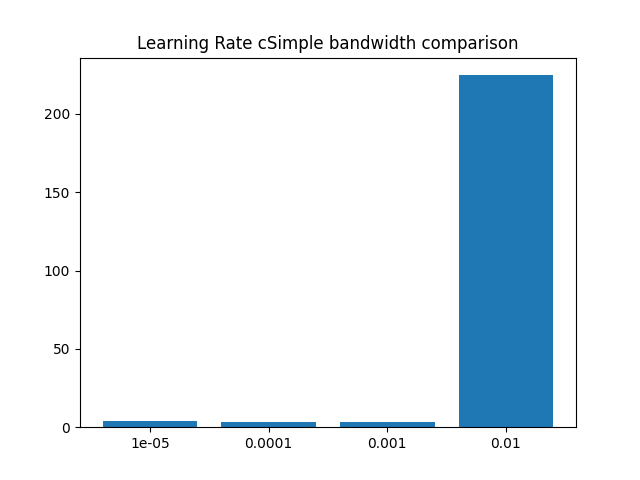
\includegraphics[width=200px]{plots/hist/a/lr/cSimple/bandwidth.png}
    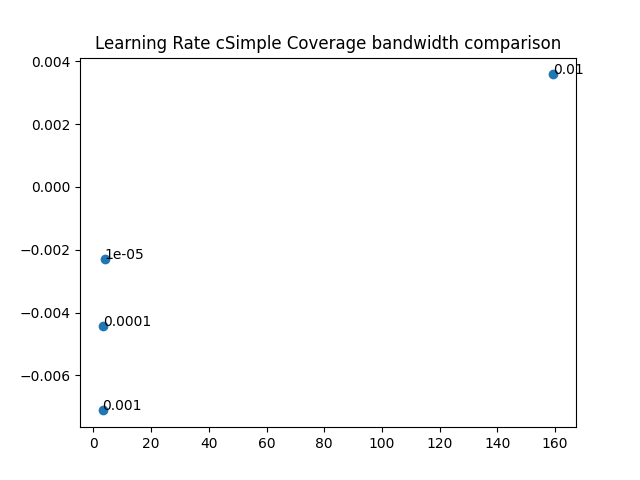
\includegraphics[width=300px]{plots/scatter/a/lr/cSimple/Coverage_bandwidth.png}
    \caption{Comparison of different learning rate (Model: Simple (Default parameter values), Epochs = 100, $\alpha$ = 0.9, Distribution = Gaussian, Config A)}
    \label{fig:comp_lr}
\end{figure}

The default learning rate in GluonTs for all deep learning models is $1^-3$

\subsubsection{Epochs} \label{comp_epochs}

\begin{figure}[!h]
    \centering
    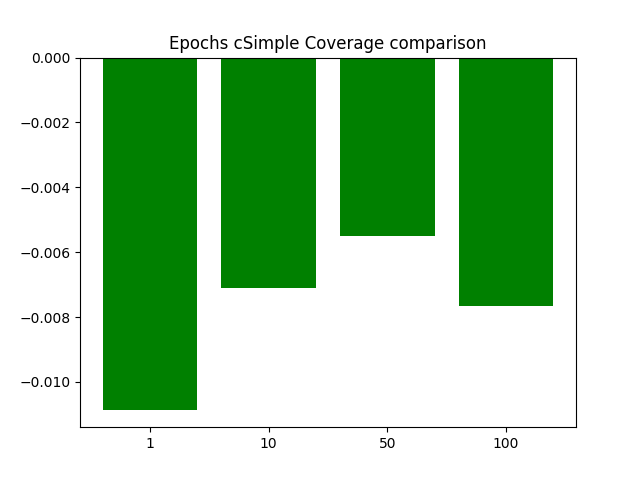
\includegraphics[width=200px]{plots/hist/a/epochs/cSimple/Coverage.png}
    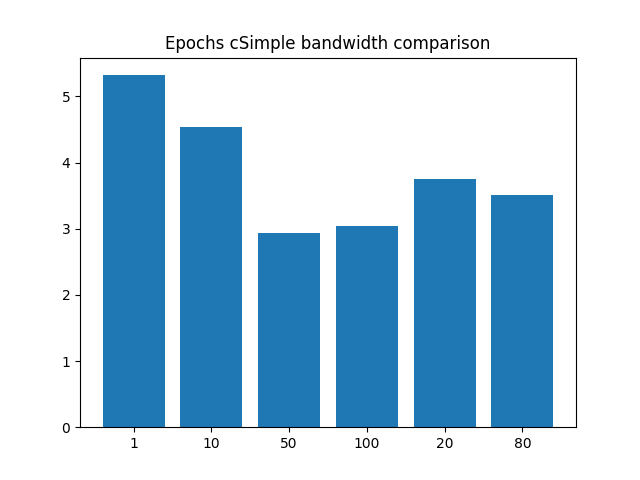
\includegraphics[width=200px]{plots/hist/a/epochs/cSimple/bandwidth.png}
    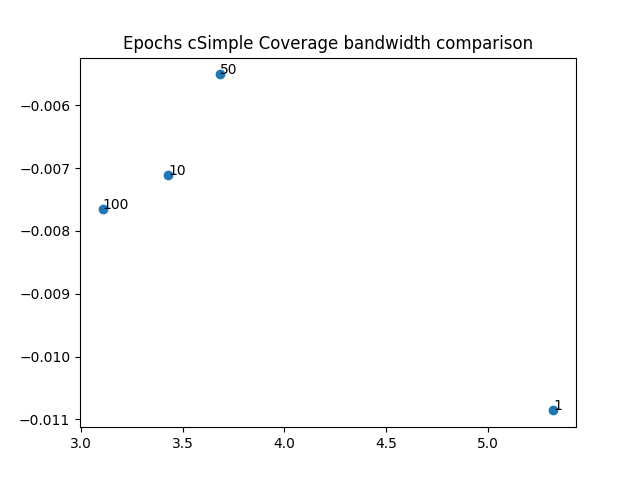
\includegraphics[width=300px]{plots/scatter/a/epochs/cSimple/Coverage_bandwidth.png}
    \caption{Comparison of different epochs number (Model: Simple (Default parameter values), $\alpha$ = 0.9, Distribution = Gaussian, Config A)}
    \label{fig:comp_epochs}
\end{figure}

All the deep learning models implemented must be trained a certain number of epochs. The default number 
is 100 epochs. 

\subsubsection{Output Distribution} \label{comp_outdistrib}

\begin{figure}[!h]
    \centering
    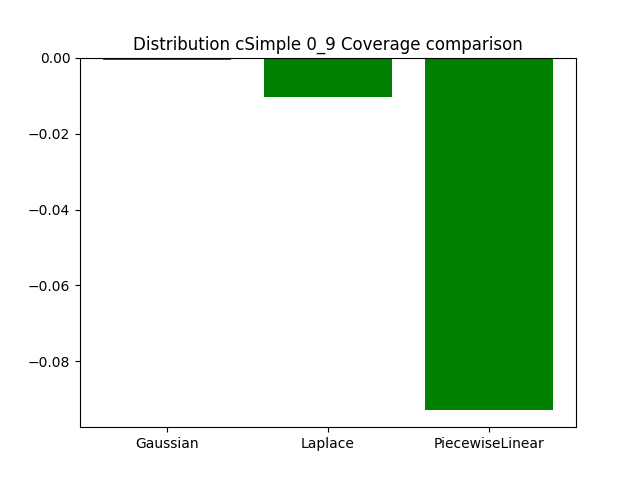
\includegraphics[width=200px]{plots/hist/a/distribution/cSimple/0_9/Coverage.png}
    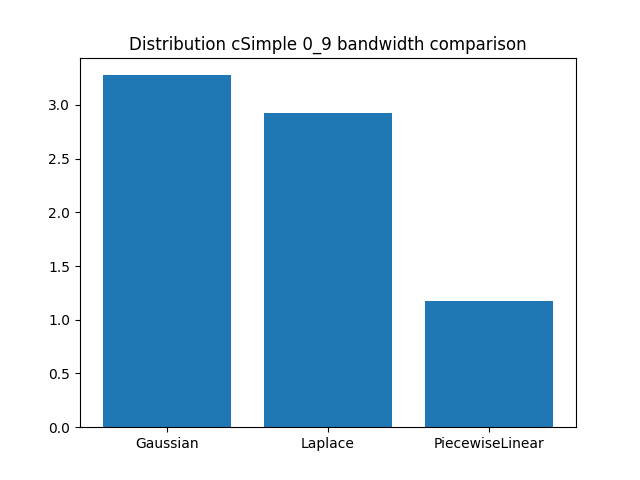
\includegraphics[width=200px]{plots/hist/a/distribution/cSimple/0_9/bandwidth.png}
    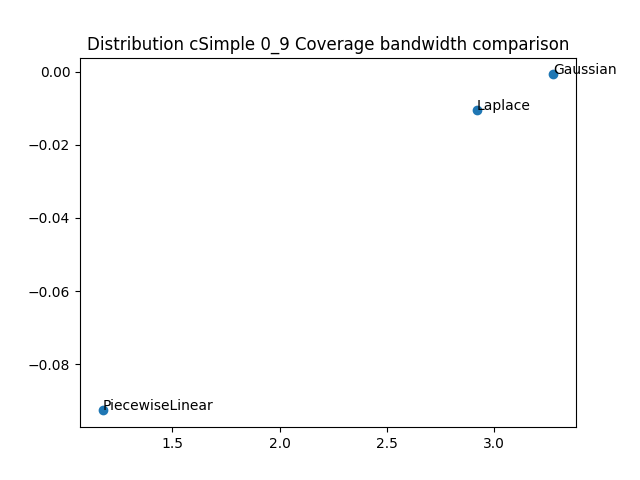
\includegraphics[width=300px]{plots/scatter/a/distribution/cSimple/0_9/Coverage_bandwidth.png}
    \caption{Comparison of different output distribution (Model: Simple (Default parameter values), Epochs = 100, $\alpha$ = 0.9,  Config A)}
    \label{fig:comp_outdistrib}
\end{figure}

As explained in section \ref{distribution} we can specify the kind of distribution that will be given as output by the models. 

\subsubsection{Alpha} \label{comp_alpha}

\begin{figure}[!h]
    \centering
    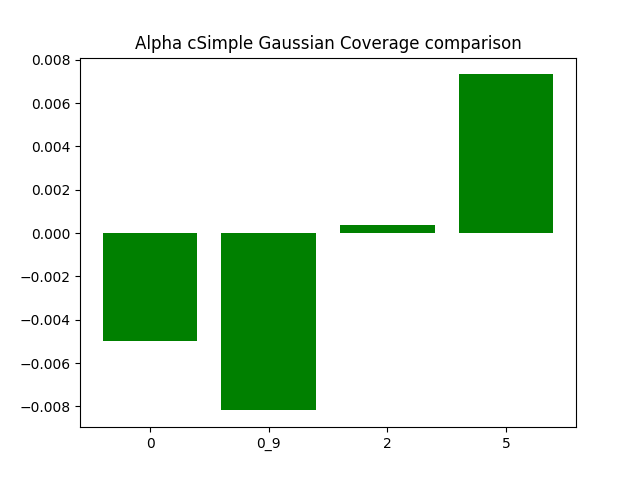
\includegraphics[width=200px]{plots/hist/a/alpha/cSimple/Gaussian/Coverage.png}
    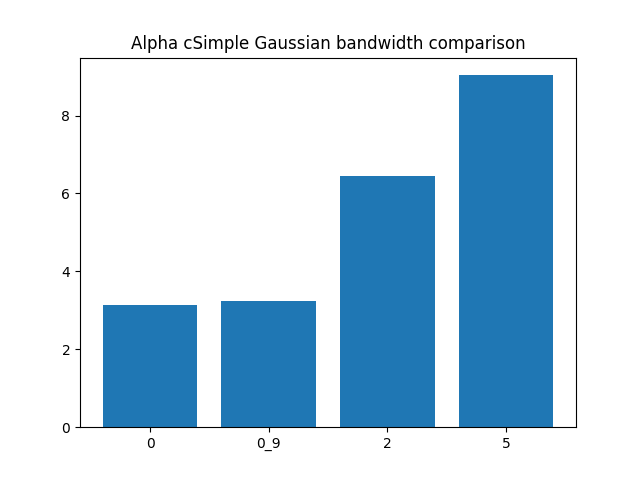
\includegraphics[width=200px]{plots/hist/a/alpha/cSimple/Gaussian/bandwidth.png}
    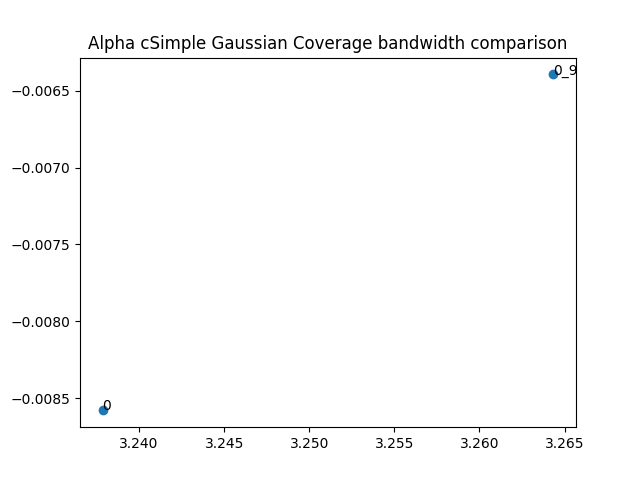
\includegraphics[width=300px]{plots/scatter/a/alpha/cSimple/Gaussian/Coverage_bandwidth.png}
    \caption{Comparison of different $\alpha$ values (Model: Simple (Default parameter values), Epochs = 100, Distribution = Gaussian, Config A)}
    \label{fig:comp_alpha}
\end{figure}

The value of $\alpha$, defined in section \ref{loss} influence the model behaviour.
Bandwidth value decrease with alpha, as Coverage increase with alpha, which tends to show that the purpose of the custom loss is observable concretely.

\subsection{Different models parameters comparison and results}

The different models are described in the \ref{diff_models} section

\subsubsection{Simple} \label{comp_simple}

\begin{figure}[!h]
    \centering
    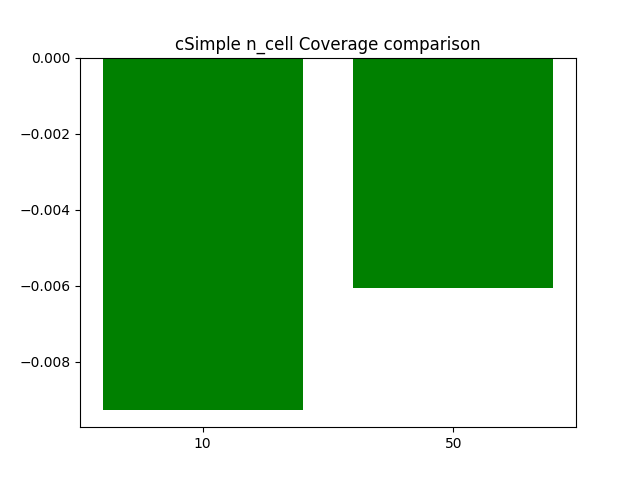
\includegraphics[width=200px]{plots/hist/a/cSimple/n_cell/Coverage.png}
    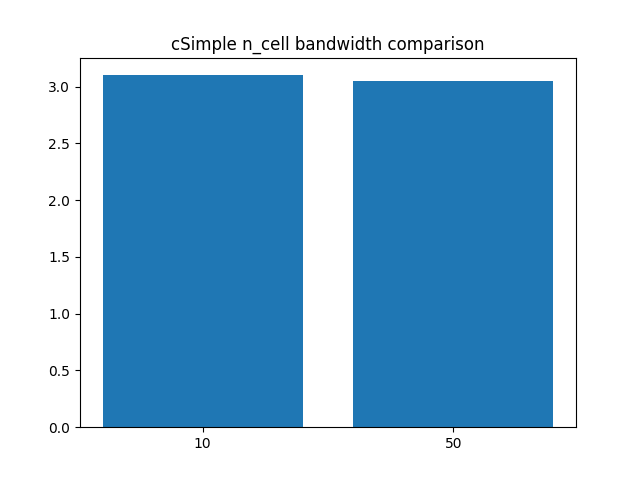
\includegraphics[width=200px]{plots/hist/a/cSimple/n_cell/bandwidth.png}
    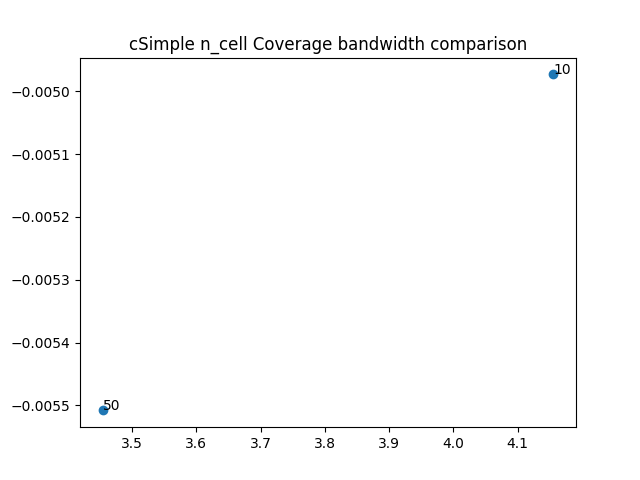
\includegraphics[width=300px]{plots/scatter/a/cSimple/n_cell/Coverage_bandwidth.png}
    \caption{Comparison of different $n\_cell$ values for Simple model (Epochs = 100, Distribution = Gaussian, $\alpha = 0.9$, Config A)}
    \label{fig:comp_simple}
\end{figure}

\begin{figure}[!h]
    \centering
    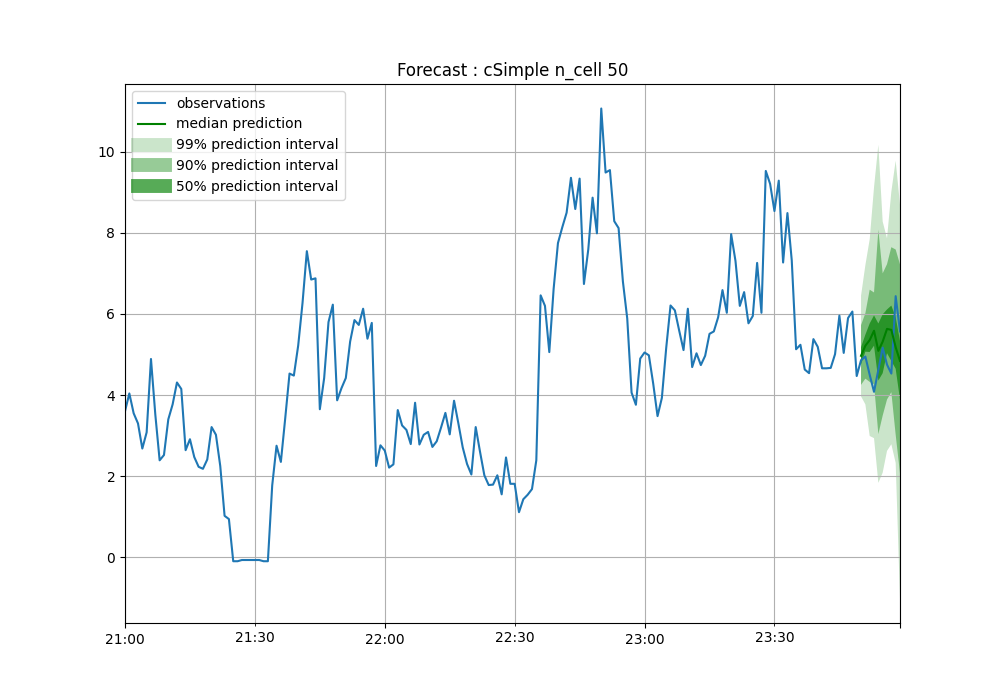
\includegraphics[width=400px]{plots/forecast/a/cSimple/n_cell/50/180.png}
    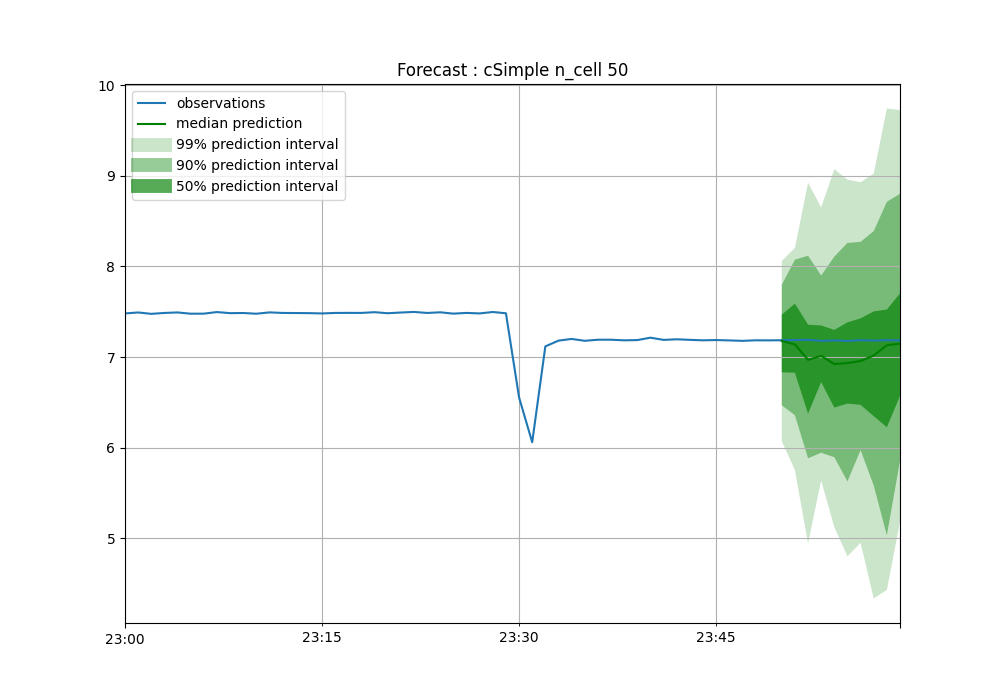
\includegraphics[width=400px]{plots/forecast/a/cSimple/n_cell/50/60.png}
    \caption{Forecast result of Simple model at 3 hours and 1 hour scale ($n\_cell = 50$ Epochs = 100, Distribution = Gaussian, $\alpha = 0.9$, Config A)}
    \label{fig:simple}
\end{figure}

The desription of this model is done in section 

\subsubsection{Simple Feed Fordward} \label{comp_feedfordward}

\begin{figure}[!h]
    \centering
    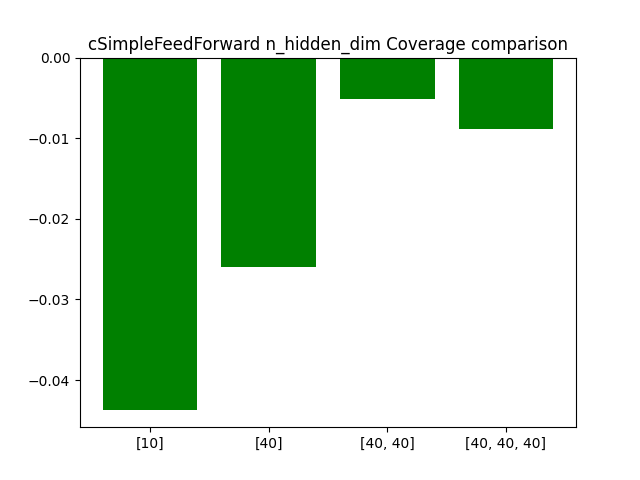
\includegraphics[width=200px]{plots/hist/a/cSimpleFeedForward/n_hidden_dim/Coverage.png}
    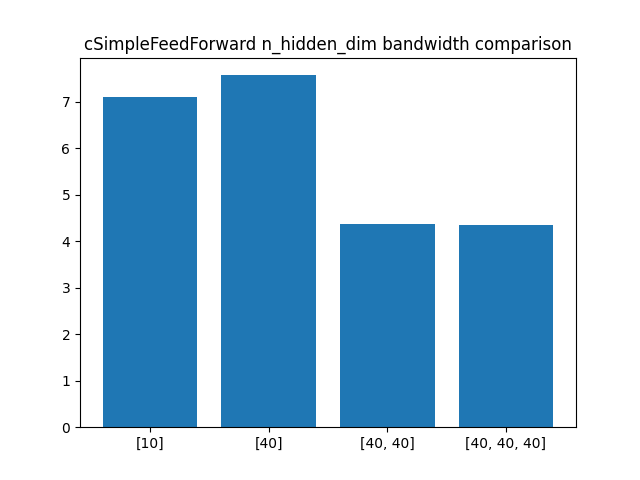
\includegraphics[width=200px]{plots/hist/a/cSimpleFeedForward/n_hidden_dim/bandwidth.png}
    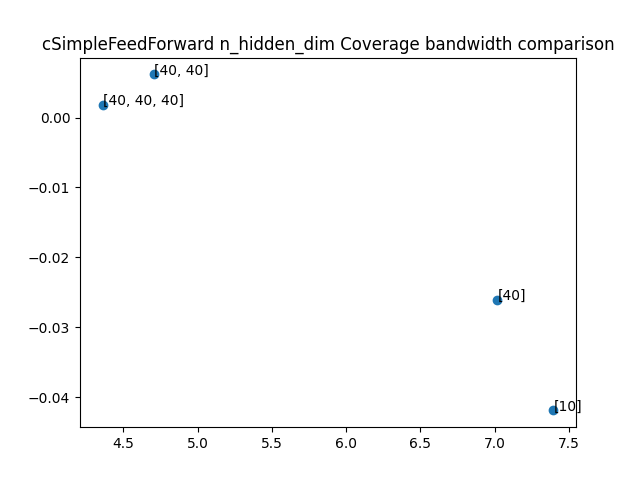
\includegraphics[width=300px]{plots/scatter/a/cSimpleFeedForward/n_hidden_dim/Coverage_bandwidth.png}
    \caption{Comparison of different $n\_hidden\_dim$ values for Simple FeedForward model (Epochs = 100, Distribution = Gaussian, $\alpha = 0.9$, Config A)}
    \label{fig:comp_feedfordward}
\end{figure}

\begin{figure}[!h]
    \centering
    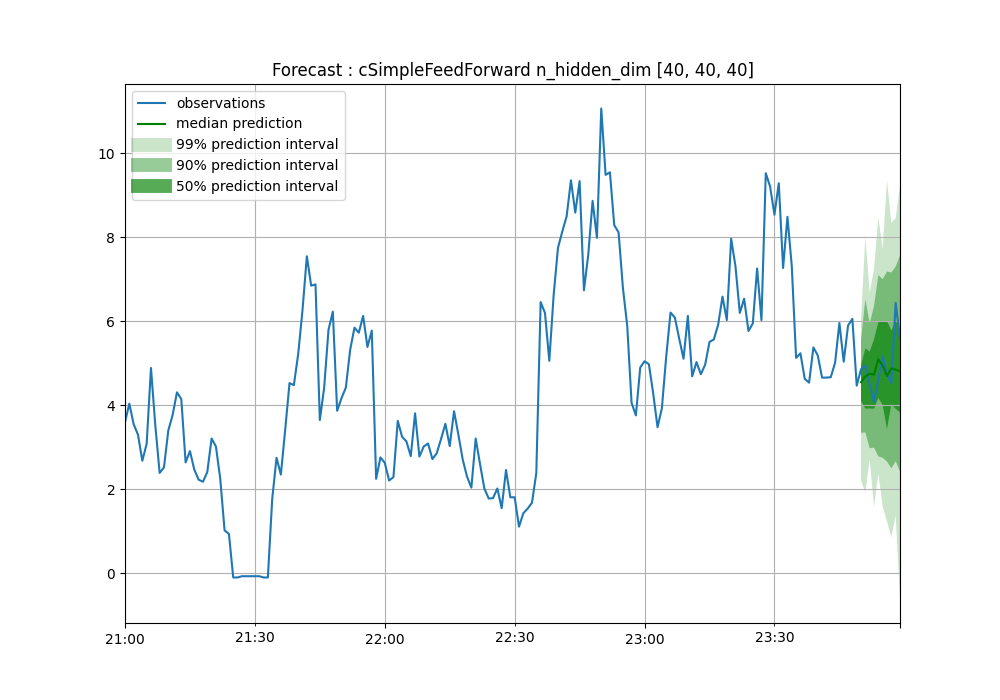
\includegraphics[width=400px]{plots/forecast/a/cSimpleFeedForward/n_hidden_dim/[40, 40, 40]/180.png}
    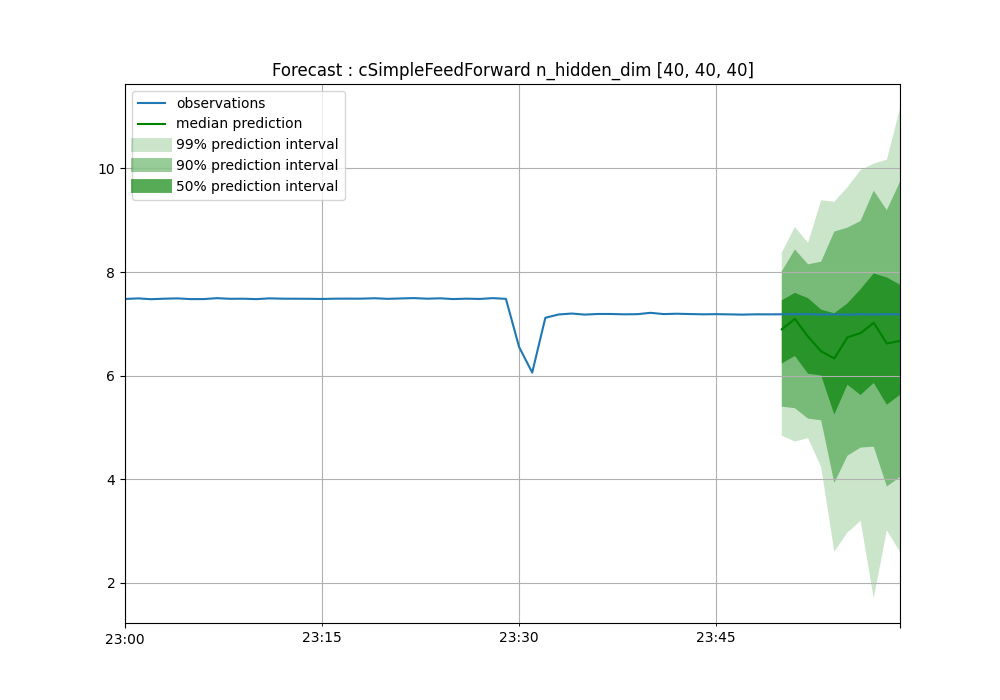
\includegraphics[width=400px]{plots/forecast/a/cSimpleFeedForward/n_hidden_dim/[40, 40, 40]/60.png}
    \caption{Forecast result of Simple FeedForward model at 3 hours and 1 hour scale ($n\_hidden_dim = [40,40,40]$ Epochs = 100, Distribution = Gaussian, $\alpha = 0.9$, Config A)}
    \label{fig:feedfordward}
\end{figure}

\subsubsection{Canonical RNN} \label{comp_canonicalrnn}

\begin{figure}[!h]
    \centering
    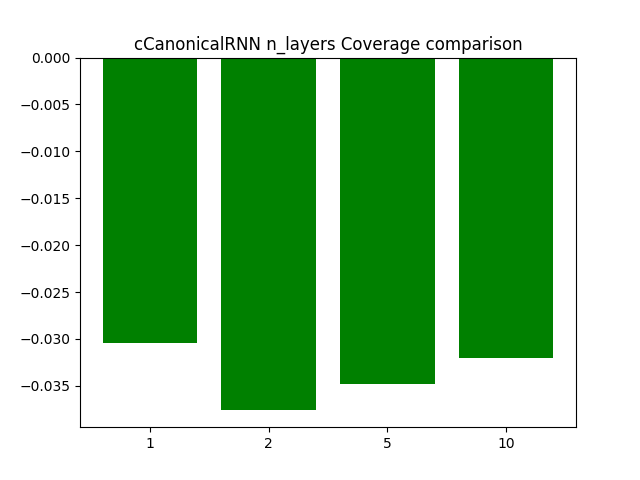
\includegraphics[width=200px]{plots/hist/a/cCanonicalRNN/n_layers/Coverage.png}
    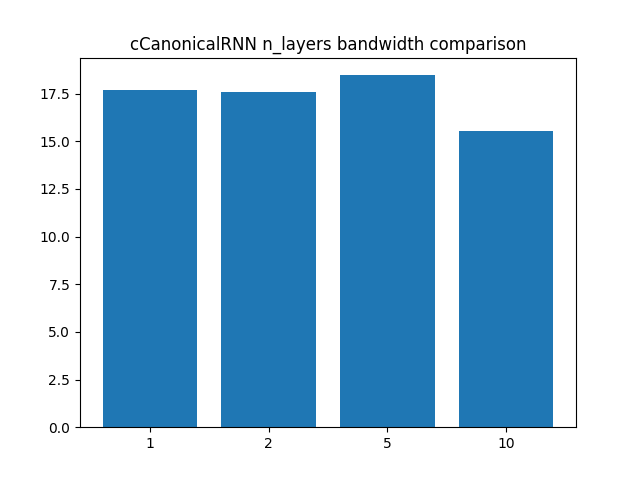
\includegraphics[width=200px]{plots/hist/a/cCanonicalRNN/n_layers/bandwidth.png}
    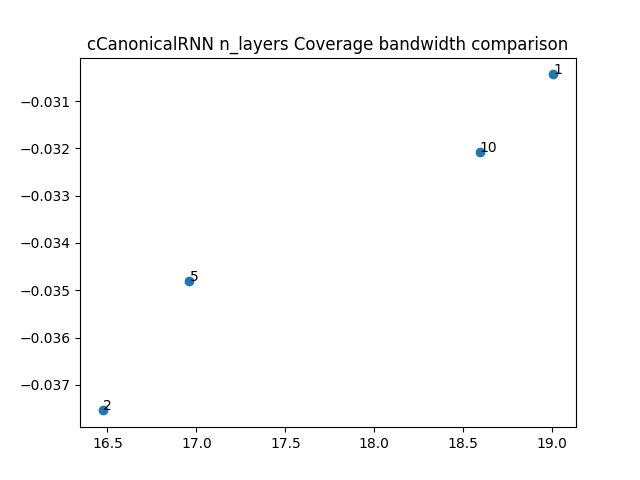
\includegraphics[width=300px]{plots/scatter/a/cCanonicalRNN/n_layers/Coverage_bandwidth.png}
    \caption{Comparison of different $n\_layers$ values for Canonical RNN model (Epochs = 100, Distribution = Gaussian, $\alpha = 0.9$, Config A)}
    \label{fig:comp_canonicalrnn}
\end{figure}

\begin{figure}[!h]
    \centering
    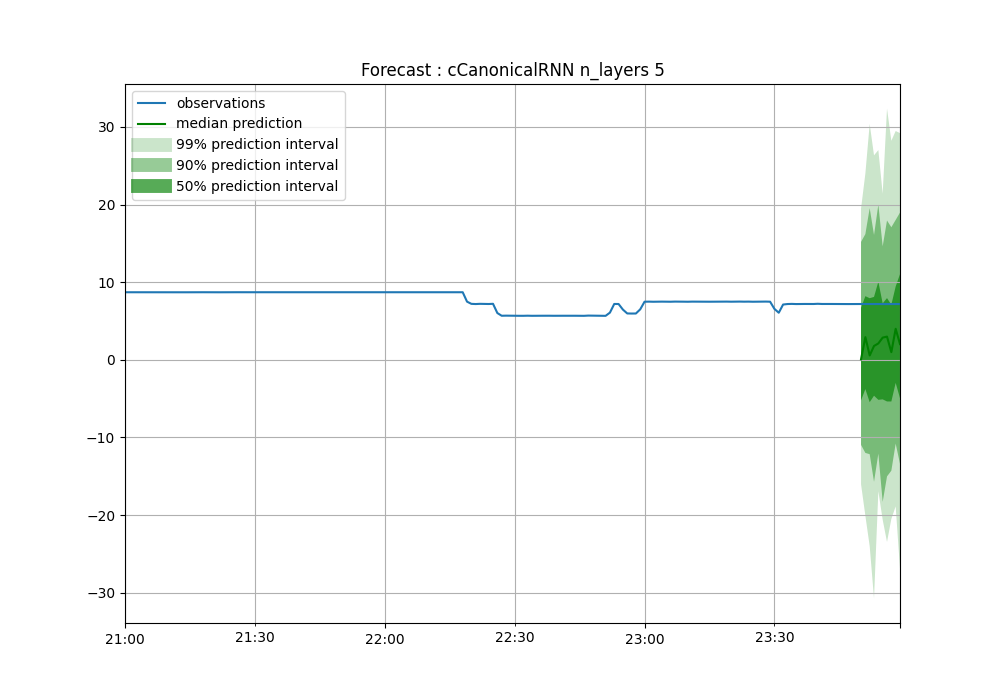
\includegraphics[width=400px]{plots/forecast/a/cCanonicalRNN/n_layers/5/180.png}
    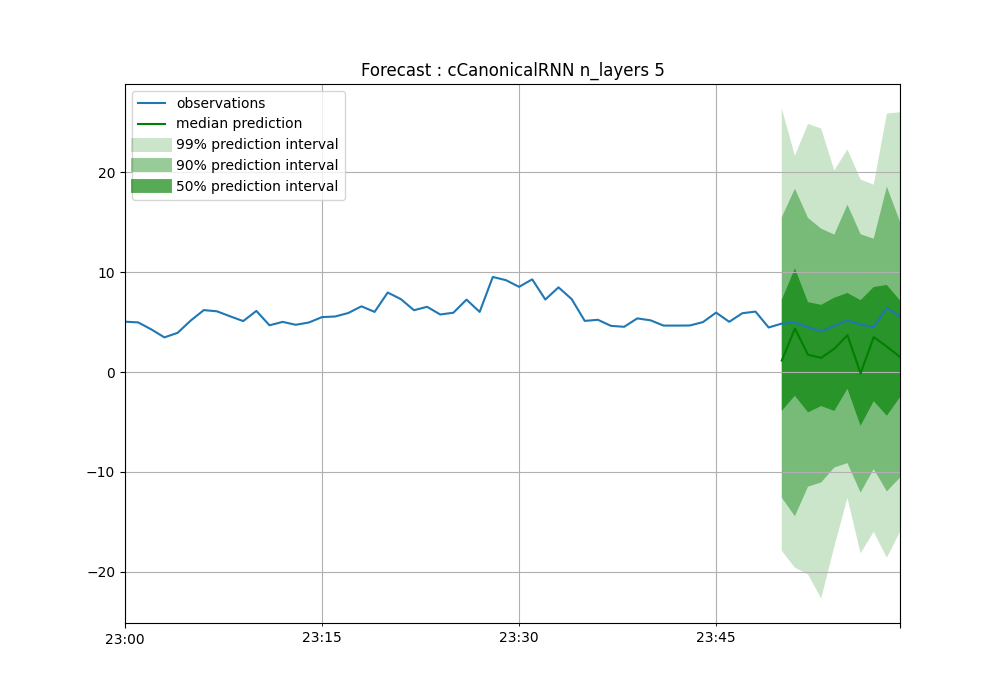
\includegraphics[width=400px]{plots/forecast/a/cCanonicalRNN/n_layers/5/60.png}
    \caption{Forecast result of Simple FeedForward model at 3 hours and 1 hour scale ($n\_layers = 5$ Epochs = 100, Distribution = Gaussian, $\alpha = 0.9$, Config A)}
    \label{fig:canonicalrnn}
\end{figure}


\subsubsection{Deep AR} \label{comp_deepar}

\begin{figure}[!h]
    \centering
    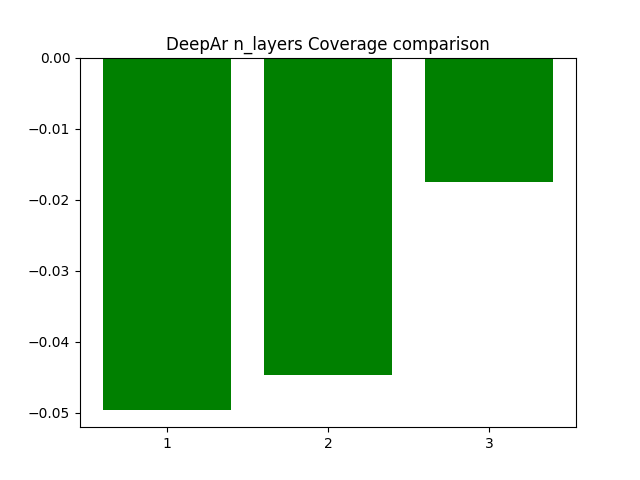
\includegraphics[width=200px]{plots/hist/a/DeepAr/n_layers/Coverage.png}
    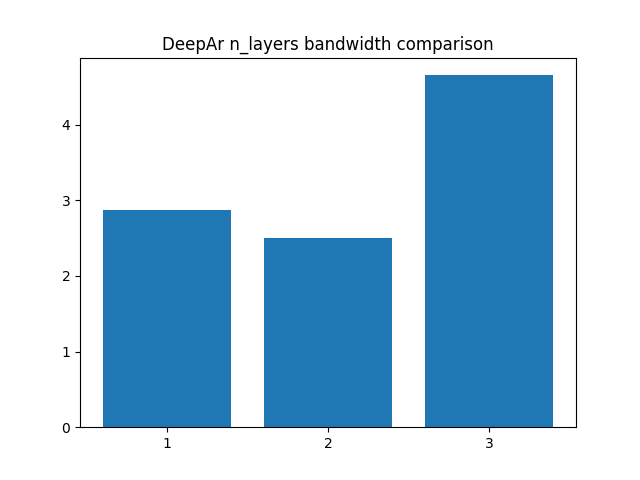
\includegraphics[width=200px]{plots/hist/a/DeepAr/n_layers/bandwidth.png}
    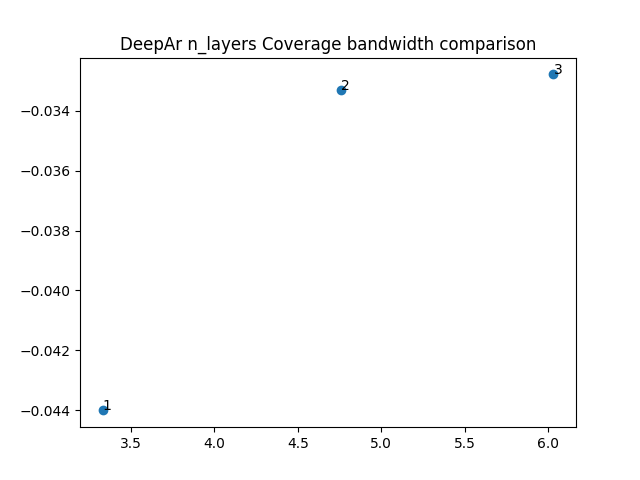
\includegraphics[width=300px]{plots/scatter/a/DeepAr/n_layers/Coverage_bandwidth.png}
    \caption{Comparison of different $n\_layers$ values for Deep AR model (Epochs = 100, Distribution = Gaussian, Config A)}
    \label{fig:comp_deepar_n_layers}
\end{figure}

\begin{figure}[!h]
    \centering
    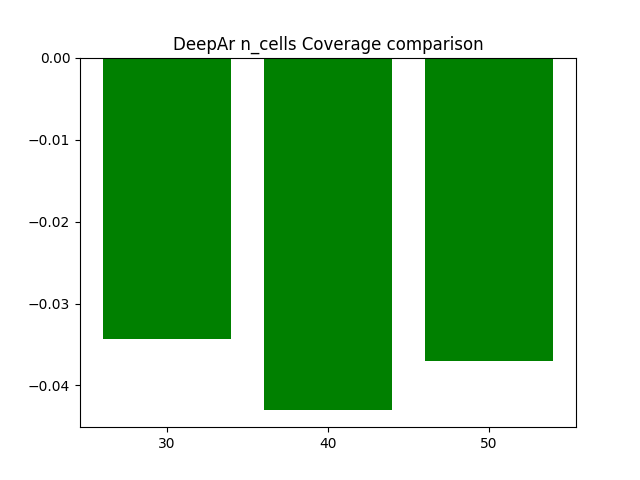
\includegraphics[width=200px]{plots/hist/a/DeepAr/n_cells/Coverage.png}
    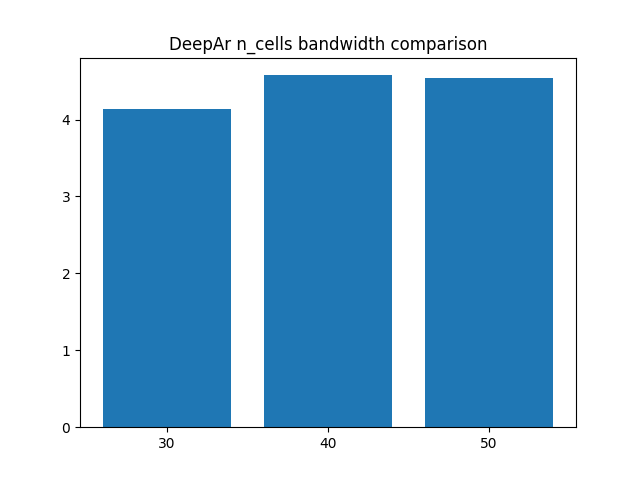
\includegraphics[width=200px]{plots/hist/a/DeepAr/n_cells/bandwidth.png}
    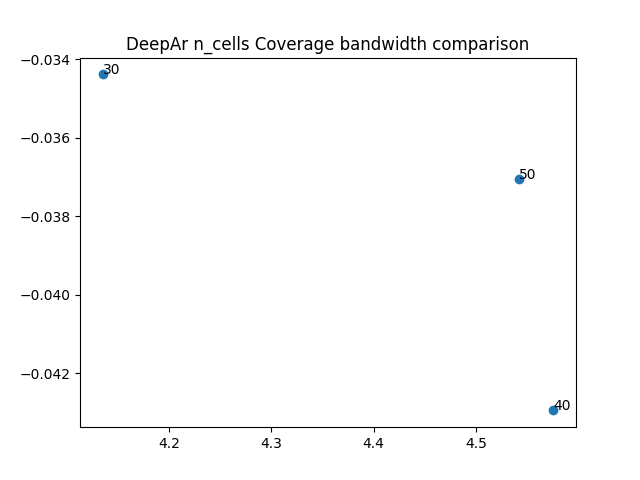
\includegraphics[width=300px]{plots/scatter/a/DeepAr/n_cells/Coverage_bandwidth.png}
    \caption{Comparison of different $n\_cells$ values for Deep AR model (Epochs = 100, Distribution = Gaussian, Config A)}
    \label{fig:comp_deepar_n_cells}
\end{figure}

\begin{figure}[!h]
    \centering
    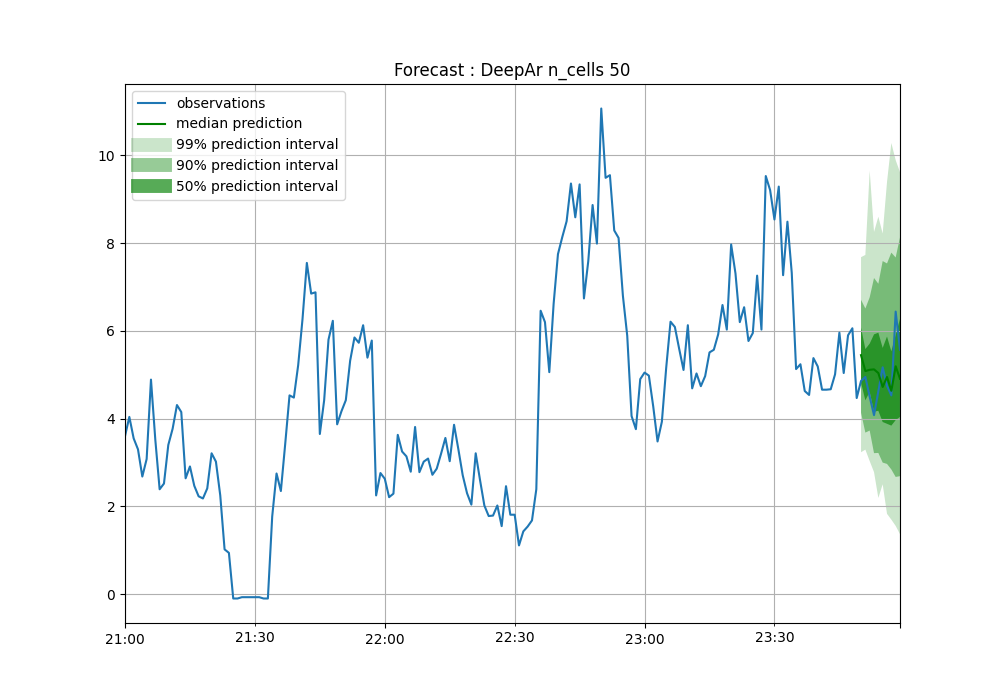
\includegraphics[width=400px]{plots/forecast/a/DeepAr/n_cells/50/180.png}
    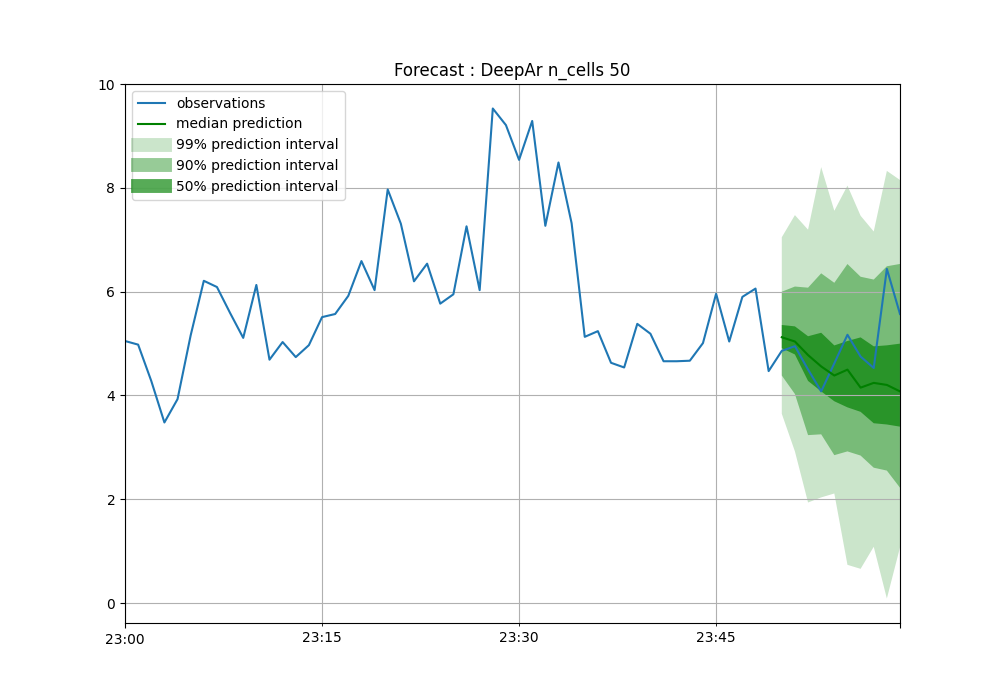
\includegraphics[width=400px]{plots/forecast/a/DeepAr/n_cells/50/60.png}
    \caption{Forecast result of Deep Ar model at 3 hours and 1 hour scale ($n\_layers = 2$, $n\_cells = 50$, Epochs = 100, Distribution = Gaussian, Config A)}
    \label{fig:deepar}
\end{figure}

\subsubsection{Deep Factor} \label{comp_deepfactor}

\begin{figure}[!h]
    \centering
    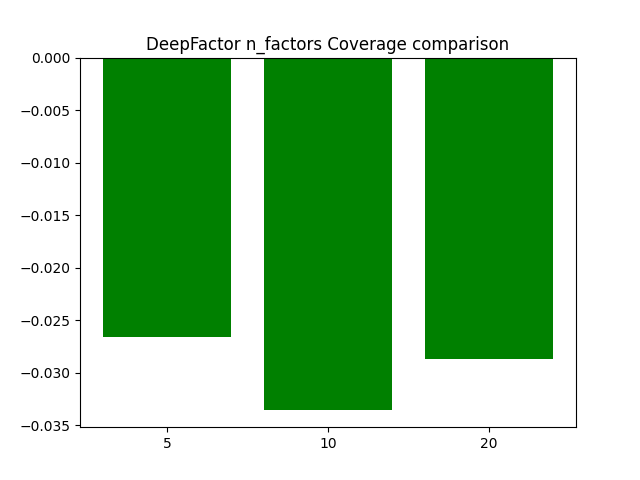
\includegraphics[width=200px]{plots/hist/a/DeepFactor/n_factors/Coverage.png}
    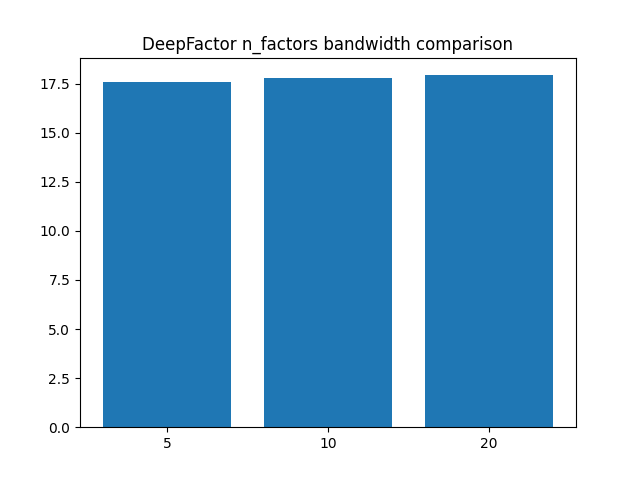
\includegraphics[width=200px]{plots/hist/a/DeepFactor/n_factors/bandwidth.png}
    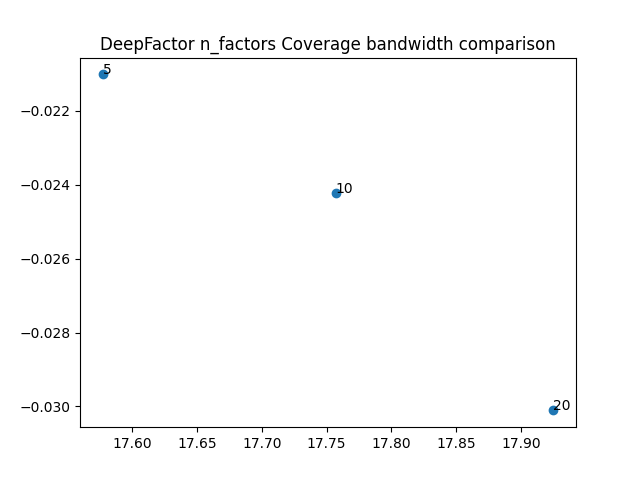
\includegraphics[width=300px]{plots/scatter/a/DeepFactor/n_factors/Coverage_bandwidth.png}
    \caption{Comparison of different $n\_factors$ values for Deep Factors model (Epochs = 100, Distribution = Gaussian, $\alpha = 0.9$, Config A)}
    \label{fig:comp_deepfactor_n_factors}
\end{figure}

\begin{figure}[!h]
    \centering
    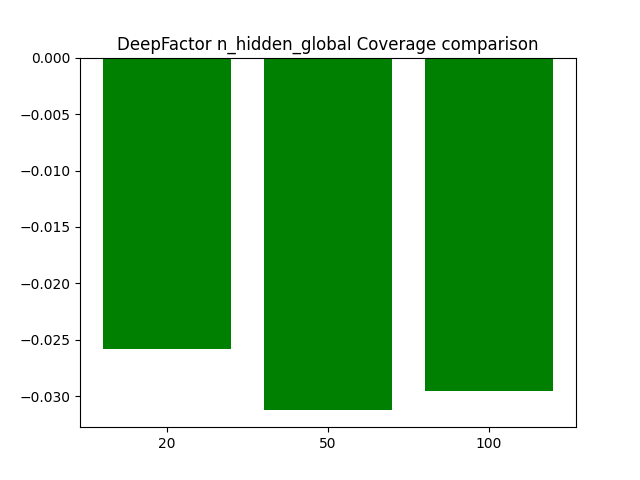
\includegraphics[width=200px]{plots/hist/a/DeepFactor/n_hidden_global/Coverage.png}
    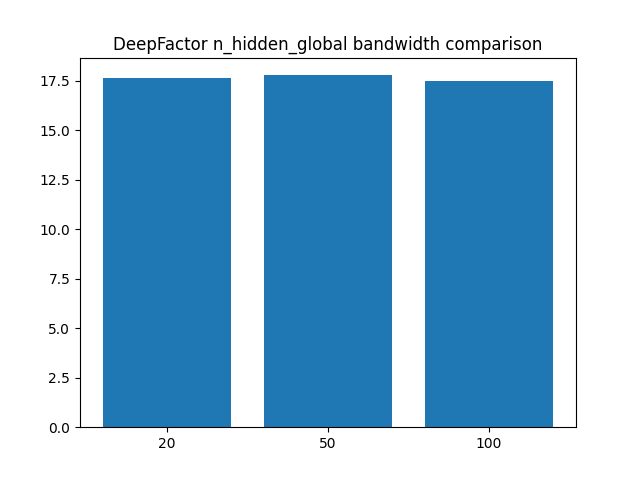
\includegraphics[width=200px]{plots/hist/a/DeepFactor/n_hidden_global/bandwidth.png}
    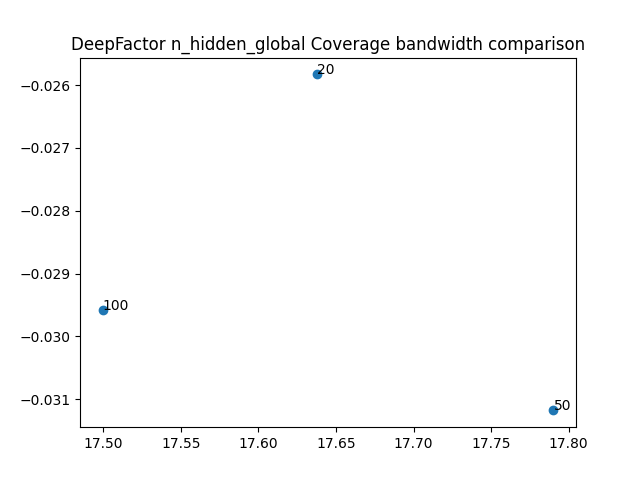
\includegraphics[width=300px]{plots/scatter/a/DeepFactor/n_hidden_global/Coverage_bandwidth.png}
    \caption{Comparison of different $n\_hidden\_global$ values for Deep Factors model (Epochs = 100, Distribution = Gaussian, $\alpha = 0.9$, Config A)}
    \label{fig:comp_deepfactor_n_hidden_globals}
\end{figure}

\begin{figure}[!h]
    \centering
    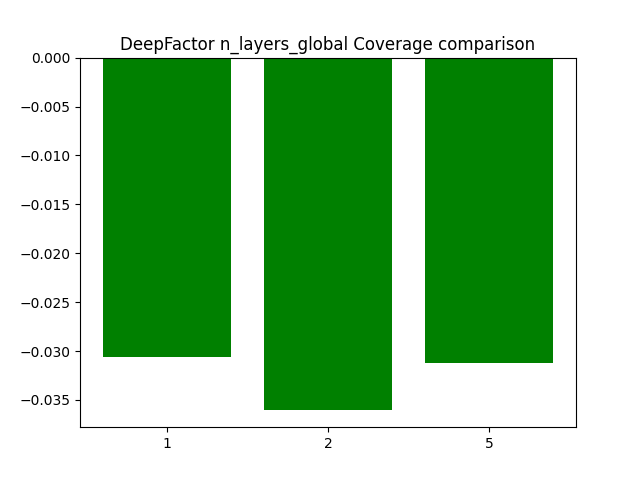
\includegraphics[width=200px]{plots/hist/a/DeepFactor/n_layers_global/Coverage.png}
    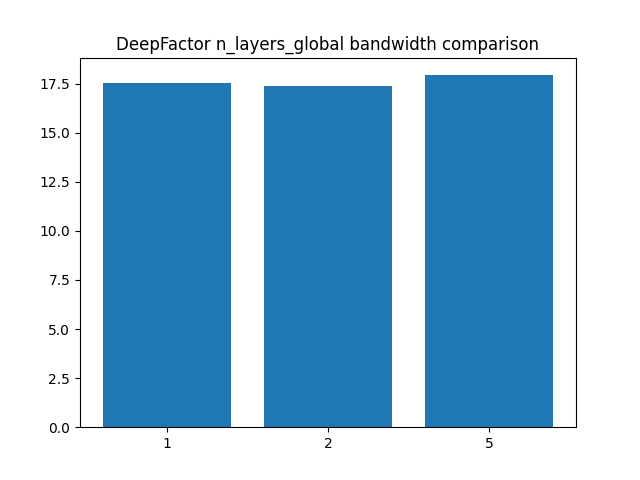
\includegraphics[width=200px]{plots/hist/a/DeepFactor/n_layers_global/bandwidth.png}
    \includegraphics[width=300px]{plots/scatter/a/DeepFactor/n_layers_global/Coverage_bandwidth.png}
    \caption{Comparison of different $n\_layers\_global$ values for Deep Factors model (Epochs = 100, Distribution = Gaussian, $\alpha = 0.9$, Config A)}
    \label{fig:comp_deepfactor_n_layers_global}
\end{figure}

\begin{figure}[!h]
    \centering
    \includegraphics[width=400px]{plots/forecast/a/DeepFactor/n_hidden_global/100/180.png}
    \includegraphics[width=400px]{plots/forecast/a/DeepFactor/n_hidden_global/100/60.png}
    \caption{Forecast result of Deep Factors model at 3 hours and 1 hour scale ($n\_factors = 5$, $n\_hidden\_global = 100$, $n\_layers\_global = 1$ Epochs = 100, Distribution = Gaussian, $\alpha = 0.9$, Config A)}
    \label{fig:comp_deepfactor_n_hidden_global}
\end{figure}

\subsubsection{MQCNN} \label{comp_mqcnn}

\begin{figure}[!h]
    \centering
    \includegraphics[width=200px]{plots/hist/a/MQCNN/mlp_final_dim/Coverage.png}
    \includegraphics[width=200px]{plots/hist/a/MQCNN/mlp_final_dim/bandwidth.png}
    \includegraphics[width=300px]{plots/scatter/a/MQCNN/mlp_final_dim/Coverage_bandwidth.png}
    \caption{Comparison of different $mlp\_final\_dim$ values for MQCNN model (Epochs = 100, Distribution = Gaussian, Config A)}
    \label{fig:comp_mqcnn}
\end{figure}

\begin{figure}[!h]
    \centering
    \includegraphics[width=400px]{plots/forecast/a/MQCNN/mlp_final_dim/40/180.png}
    \includegraphics[width=400px]{plots/forecast/a/MQCNN/mlp_final_dim/40/60.png}
    \caption{Forecast result of MQCNN model at 3 hours and 1 hour scale ($mlp\_final\_dim = 40 $, Epochs = 100, Distribution = Gaussian, Config A)}
    \label{fig:mqcnn}
\end{figure}

\subsubsection{MQRNN} \label{comp_mqrnn}

\begin{figure}[!h]
    \centering
    \includegraphics[width=200px]{plots/hist/a/MQRNN/mlp_final_dim/Coverage.png}
    \includegraphics[width=200px]{plots/hist/a/MQRNN/mlp_final_dim/bandwidth.png}
    \includegraphics[width=300px]{plots/scatter/a/MQRNN/mlp_final_dim/Coverage_bandwidth.png}
    \caption{Comparison of different $mlp\_final\_dim$ values for MQRNN model (Epochs = 100, Distribution = Gaussian, Config A)}
    \label{fig:comp_mqrnn}
\end{figure}

\begin{figure}[!h]
    \centering
    \includegraphics[width=400px]{plots/forecast/a/MQRNN/mlp_final_dim/20/180.png}
    \includegraphics[width=400px]{plots/forecast/a/MQRNN/mlp_final_dim/20/60.png}
    \caption{Forecast result of MQRNN model at 3 hours and 1 hour scale ($mlp\_final\_dim = 20 $, Epochs = 100, Distribution = Gaussian, Config A)}
    \label{fig:mqrnn}
\end{figure}


\subsubsection{Gaussian Process} \label{comp_gp}

\begin{figure}[!h]
    \centering
    \includegraphics[width=400px]{plots/forecast/a/model/Gaussian/0_9/GaussianProcess/180.png}
    \includegraphics[width=400px]{plots/forecast/a/model/Gaussian/0_9/GaussianProcess/60.png}
    \caption{Forecast result of Gaussian Process model at 3 hours and 1 hour scale (, Epochs = 100, Distribution = Gaussian, Config A)}
    \label{fig:gp}
\end{figure}


\subsubsection{NPTS} \label{comp_npts}

\begin{figure}[!h]
    \centering
    \includegraphics[width=400px]{plots/forecast/a/model/Gaussian/0_9/NPTS/180.png}
    \includegraphics[width=400px]{plots/forecast/a/model/Gaussian/0_9/NPTS/60.png}
    \caption{Forecast result of NPTS model at 3 hours and 1 hour scale (Epochs = 100, Config A)}
    \label{fig:npts}
\end{figure}

\subsubsection{ETS} \label{comp_ets}

\begin{figure}[!h]
    \centering
    \includegraphics[width=400px]{plots/forecast/a/model/Gaussian/0_9/NPTS/180.png}
    \includegraphics[width=400px]{plots/forecast/a/model/Gaussian/0_9/NPTS/60.png}
    \caption{Forecast result of ETS model at 3 hours and 1 hour scale (Epochs = 100, Config A)}
    \label{fig:ets}
\end{figure}

\subsection{Global comparison}

\begin{figure}[!h]
    \centering
    \includegraphics[width=200px]{plots/hist/a/model/0_9/Gaussian/Coverage.png}
    \includegraphics[width=200px]{plots/hist/a/model/0_9/Gaussian/bandwidth.png}
    \includegraphics[width=300px]{plots/scatter/a/model/0_9/Gaussian/Coverage_bandwidth.png}
    \caption{Comparison of different models (Epochs = 100, Distribution = Gaussian, Config A)}
    \label{fig:comp_mqcnn}
\end{figure}



\end{document}
